%============================================================================%
% Antoine Gé́ré (gereantoine@gmail.com). 
%============================================================================%                                                     

%-- CLASS ------------------------------------------------------------------%

\documentclass[9pt]{beamer} 

\pdfoutput=1 

\makeatletter 

%-- PACKAGES ----------------------------------------------------------------%

\usepackage{amscd}
\usepackage{amsmath}
\usepackage{amsthm}
\usepackage{amsxtra}
\usepackage{array} 

\usepackage[english]{babel} 

\usepackage{cancel}
\usepackage{color}

\usepackage{enumitem}

\usepackage{fancyhdr}
\usepackage[T1]{fontenc} 

\usepackage{geometry} 
\usepackage{graphicx} 

\usepackage{hyperref} 

\usepackage[utf8]{inputenc} 

\usepackage{letltxmacro}
\usepackage{lmodern}

\usepackage{manfnt}
\usepackage{multicol} 

\usepackage[numbers,sort]{natbib}

\usepackage{pgf}

\usepackage{setspace} 

\usepackage{tikz}

\usepackage{url}
 
\usepackage{wasysym}
\usepackage{wrapfig}

\usepackage{xcolor}

%-- THEME -------------------------------------------------------------------%

\mode<presentation>
{

  %== NAVIGATION SYMBOLS ======================================================%    

  \setbeamertemplate{navigation symbols}{}
  
  %== TITLE PAGE ==============================================================%    

  \newcommand\coauthor[1]{\def\insertcoauthor{#1}}
  \coauthor{}

  \newcommand\conference[1]{\def\insertconference{#1}}
  \conference{}

  \newcommand\shortconference[1]{\def\insertshortconference{#1}}
  \shortconference{}

  \newcommand\paper[1]{\def\insertpaper{#1}}
  \paper{}

  \newcommand\LogoUniv[1]{\def\insertLogoUniv{#1}}
  \paper{}
  
  \newcommand\TitlePic[1]{\def\insertTitlePic{#1}}
  \paper{}

  \pgfdeclareverticalshading[title page.bg]{beamer@titleshade}{\paperwidth}{%
    color(0pt)=(black!30!white);
    color(3pt)=(black!60!white);
    color(3pt)=(title page.bg);
    color(113pt)=(title page.bg);
    color(113pt)=(black!60!white);
    color(116pt)=(black!30!white)}
  
  \defbeamertemplate*{title page}{gottingen14}[1][]
  {%
    \hbox{%
      %
      \leavevmode%
      \advance\beamer@leftmargin by -12bp%
      \advance\beamer@rightmargin by -12bp%
      \beamer@tempdim=\textwidth%
      \advance\beamer@tempdim by \beamer@leftmargin%
      \advance\beamer@tempdim by \beamer@rightmargin%
      \hskip-\Gm@lmargin%
      %
      \hbox{%
	\setbox%
	\beamer@tempbox=\hbox{%
	%
	\begin{minipage}[b]{\paperwidth}%
	  \vbox{}%
	  \leavevmode%
	  \center{%
	    {\usebeamerfont{title}\inserttitle}\\[5pt]%
	    {\usebeamerfont{author}\color{black}\insertauthor}\\[1pt]%
	    %\insertLogoUniv
	    {\usebeamerfont{institute}\color{black}\insertinstitute}\\[-2pt]%
	    {\usebeamerfont{conference}\color{black}\insertconference, \insertdate}\\[1pt]%
	    {\usebeamerfont{coauthor}\color{black} joint work with \insertcoauthor}\\[-3pt]%
	    {\usebeamerfont{paper}\color{black}\insertpaper}%
	  }%
	  \strut%
	  \par%
	  \vbox{}%
	\end{minipage}%
	}%
	%
	\beamer@tempdim=\ht\beamer@tempbox%
	\advance\beamer@tempdim by 125pt%
	%
	\begin{pgfpicture}{0pt}{0pt}{\paperwidth}{\beamer@tempdim}
	  \pgfsetfillopacity{0.8}
	  \pgftext[left,base]{\pgfuseshading{beamer@titleshade}}
	\end{pgfpicture}
	%
	\hskip-\paperwidth%
	\box\beamer@tempbox%
      }%
    }%
  }

  %== TEMPLATE ================================================================% 
 
  \setbeamertemplate{title page}[gottingen14][colsep=-4bp,rounded=false]
  \setbeamertemplate{sections/subsections in toc}[ball]
  \setbeamertemplate{items}[ball]
  \setbeamertemplate{blocks}[default]
  \setbeamertemplate{part page}[default][colsep=-4bp,rounded=false]
    
  %== COLOR ===================================================================% 
  
  \setbeamercolor{title page}{bg=white!96!black,fg=red!62!black}
  \setbeamercolor{frametitle}{bg=white,fg=red!60!black}
  \setbeamercolor{subsection in head/foot}{bg=white!95!black,fg=red!60!black}
  \setbeamercolor{author in head/foot}{bg=white,fg=red!60!black}
  \setbeamercolor{title in head/foot}{bg=white,fg=red!60!black}
  \setbeamercolor{normal text}{black}
  \setbeamercolor{headline@color}{bg=black,fg=green}
  \setbeamercolor{block title}{bg=black!20!white,fg=white}
  \setbeamercolor{block body}{bg=black!20!white,fg=black}
  \setbeamercolor{block body alerted}{bg=black!40!white,fg=black}
  \setbeamercolor{block title alerted}{bg=black!40!white,fg=black}
  \setbeamercolor{block body example}{bg=black!10!white,fg=black}
  \setbeamercolor{block title example}{bg=black!10!white,fg=black}
  \setbeamercolor{button}{bg=black!50!white,fg=white}
  \setbeamercolor{sidebar}{bg=black,fg=white}
  \setbeamercolor{palette sidebar primary}{bg=black,fg=white}
  \setbeamercolor{palette sidebar secondary}{bg=black,fg=white}
  \setbeamercolor{palette sidebar tertiary}{bg=black,fg=white}
  \setbeamercolor{palette sidebar quaternary}{bg=black,fg=white}
  \setbeamercolor{titlelike}{bg=green,fg=white}
  \setbeamercolor{separation line}{white}
  \setbeamercolor{fine separation line}{white}

  %== FONT ====================================================================% 
  
  \setbeamerfont{frametitle}{size={\normalsize},series={\bf}}
  \setbeamerfont{block title}{size={\scriptsize},series={}}
  \setbeamerfont{block body}{size={},series={}}
  \setbeamerfont{block title example}{size={\normalsize},series={}}
  \setbeamerfont{block body example}{size={},series={}}
  \setbeamerfont{title}{size={\LARGE},series={\bf}}
  \setbeamerfont{author}{size={\Large},series={\bf}}
  \setbeamerfont{institute}{size={\normalsize},series={}}
  \setbeamerfont{conference}{size={\large},series={}}
  \setbeamerfont{date}{size={\normalsize},series={}}
  \setbeamerfont{coauthor}{size={\normalsize},series={\bf}}
  \setbeamerfont{paper}{size={\normalsize},series={\tt}}

  %== COVERED =================================================================% 
  
  \setbeamercovered{transparent}
    
  %== SHADOWS =================================================================% 

  \AtBeginDocument{%
    \pgfdeclareverticalshading{beamer@topshade}{\paperwidth}{%
      color(0pt)=(bg);%
      color(4pt)=(black!50!bg)}%
    \pgfdeclareverticalshading{beamer@bottomshade}{\paperwidth}{%
      color(0pt)=(black!50!bg);%
      color(4pt)=(bg)}%
    \pgfdeclarehorizontalshading{beamer@rightshade}{\paperwidth}{%
      color(0pt)=(black!50!bg);%
      color(4pt)=(bg)}%
    \pgfdeclarehorizontalshading{beamer@leftshade}{\paperwidth}{%
      color(0pt)=(black!50!bg);%
      color(4pt)=(bg)}%
  }%

  %== FRAME TITLE =============================================================% 

    \pgfdeclareverticalshading[frametitle.bg]{beamer@frametitleshade}{\paperwidth}
    {%
      color(0pt)=(frametitle.bg);
      color(36pt)=(frametitle.bg)
    }%

    \defbeamertemplate*{frametitle}{nosplit theme}
    {%
      \nointerlineskip%
      \vskip-2.5pt%
      \hbox{\leavevmode
        \advance\beamer@leftmargin by -12bp%
        \advance\beamer@rightmargin by -12bp%
        \beamer@tempdim=\textwidth%
        \advance\beamer@tempdim by \beamer@leftmargin%
        \advance\beamer@tempdim by \beamer@rightmargin%
        \hskip-\Gm@lmargin\hbox{%
          \setbox\beamer@tempbox=\hbox{
          \begin{minipage}[b]{\paperwidth}%
              \vbox{}%
              \vskip0ex%
              \leftskip0.3cm%
              \rightskip0.3cm plus1fil\leavevmode
              \insertframetitle%
              \ifx\insertframesubtitle\@empty%
                \strut\par%
              \else
                \par{\usebeamerfont*{framesubtitle}{\insertframesubtitle}\strut\par}%
              \fi%
              \vskip5pt%
              \nointerlineskip
              \vbox{}%
              \end{minipage}}%
          \beamer@tempdim=\ht\beamer@tempbox%
          \advance\beamer@tempdim by 2pt%
          \begin{pgfpicture}{0pt}{0pt}{\paperwidth}{\beamer@tempdim}
            \usebeamercolor{frametitle}
            \pgfpathrectangle{\pgfpointorigin}{\pgfpoint{\paperwidth}{\beamer@tempdim}}
            \pgfusepath{clip}
            \pgftext[left,base]{\pgfuseshading{beamer@frametitleshade}}
          \end{pgfpicture}
          \hskip-\paperwidth%
          \box\beamer@tempbox%
        }%
        \hskip-\Gm@rmargin%
      }%
      \nointerlineskip
        \vskip-0.2pt
        \hbox to\textwidth{\hskip-\Gm@lmargin\pgfuseshading{beamer@topshade}\hskip-\Gm@rmargin}
        \vskip-2pt
    }
    
  %== FOOTLINE ================================================================%    

  \newcommand{\backupbegin}{
    \newcounter{framenumberappendix}
    \setcounter{framenumberappendix}{\value{framenumber}}
  }

  \newcommand{\backupend}{
    \addtocounter{framenumberappendix}{-\value{framenumber}}
    \addtocounter{framenumber}{\value{framenumberappendix}} 
  }

  \defbeamertemplate*{footline}{nosplit theme}{%
    \vskip1pt
    \pgfuseshading{beamer@bottomshade}
    \vskip1.5pt
    \leavevmode%
    \hbox{%
      \begin{beamercolorbox}[wd=.2\paperwidth,center]{footline@color}%
	\usebeamerfont{author in head/foot} \insertauthor
      \end{beamercolorbox}%
      \begin{beamercolorbox}[wd=.2\paperwidth,center]{footline@color}%
	\usebeamerfont{institute in head/foot} \insertshortconference
      \end{beamercolorbox}%
      \begin{beamercolorbox}[wd=.5\paperwidth,center]{footline@color}%
	\usebeamerfont{title in head/foot} \inserttitle 
      \end{beamercolorbox}%
      \begin{beamercolorbox}[wd=.1\paperwidth,center]{footline@color}%
	\insertframenumber{} / \inserttotalframenumber 
      \end{beamercolorbox}%
    }%
    \vskip0.5pt%
  }%
%
}%
%
\mode%
%
<all>

%-- COMMANDS ----------------------------------------------------------------%

\newcommand{\bra}[1]{\langle{#1}|} % Define the Bra.       
\newcommand{\ket}[1]{|{#1}\rangle} % Define the Ket.

\newcommand{\Bracket}[2]{\langle #1 | #2 \rangle} % Define the bracket
\newcommand{\PB}[1]{\left\{{#1}\right\}} % Define the Poisson bracket.
\newcommand{\Comut}[1]{\left[ #1 \right]} % Define the commutator.

\newcommand{\Tdot}{\cdot_\Tsf} % Define the symbol for the general time ordering product.
\newcommand{\TdotH}{\cdot_{\Tsf_\Hsf}} % Define the symbol for the time ordering product defined for H.

\newcommand{\Smearip}[1]{\left\langle #1 \right\rangle} % Define the smearing product.

\newcommand{\abs}[1]{\left|{#1}\right|} % Define the absolute value.
\newcommand{\norm}[1]{\left|{#1}\right|} % Definie the norm.
\newcommand{\dmu}[1]{\dsf\mu_{#1}} % Definie the symbol for the measure.

\newcommand{\expo}{\mathsf{exp}} % Define the exponential exp.
\newcommand{\E}{\mathsf{e}} % Define the exponential e.
\newcommand{\logar}{\mathsf{log}} % Define the logarithm.
\renewcommand{\sin}{\mathsf{sin}} % Redefine the sinus.
\renewcommand{\cos}{\mathsf{cos}} % Redefine the cosinus.
\renewcommand{\tan}{\mathsf{tan}} % Redefine the tangent.
\renewcommand{\arcsin}{\mathsf{arcsin}} % Redefine the arcsinus.
\renewcommand{\arccos}{\mathsf{arccos}} % Redefine the arccosinus.
\renewcommand{\arctan}{\mathsf{arctan}} % Redefine the arctangent.

\renewcommand{\inf}{\mathsf{inf}} % Redefine the inf.
\renewcommand{\sup}{\mathsf{sup}} % Redefine the sup.
\renewcommand{\deg}{\mathsf{deg}} % Redefine the degree of a polynom.

\renewcommand{\arg}{\mathsf{arg}} % Redefine the argument.
\newcommand{\Arg}{\mathsf{Arg}} % Redefine the principal value of the\cite[p.646]{BF2000} argument.

\renewcommand{\Re}{\mathsf{Re}} % Define the real part.
\renewcommand{\Im}{\mathsf{Im}} % Define the imaginary part.

\newcommand{\pp}{\mathsf{pp}} % Define the principal part.
\newcommand{\rp}{\mathsf{rp}} % Define the regular part.

\newcommand{\pv}{\mathsf{pv}} % Define the principal value.

\renewcommand{\det}{\mathsf{det}} % Redefine the determinant.
\newcommand{\tr}{\mathsf{Tr}} % Define the trace.

\newcommand{\cg}[6]{\left(\begin{array}{cc|c} #1 & #3 & #5 \\ #2 & #4 & #6 \end{array}\right)} % Define the symbole for Clebsch Gordan coefficients.
\newcommand{\wig}[6]{\left(\begin{array}{ccc} #1 & #3 & #5 \\ #2 & #4 & #6 \end{array}\right)} % Define the symbole for the 3-j (Wigner symbols).

\newcommand{\wick}[1]{:\!{#1}\!:} % Define the wick product.

\newcommand{\WF}{\mathsf{WF}} % Define the wave front set.
\newcommand{\supp}{\mathsf{supp}} % Define the support.
\newcommand{\Smatrix}{\mathbf{\mathsf{S}}}% Define the S matrix.

\newcommand{\sd}{\mathsf{sd}} % Define the scaling degree.
\renewcommand{\div}{\mathsf{div}} % Redefine the divergence degree.

\newcommand{\EndDfn}{\hfill\ensuremath{\blacktriangleright}} % Define the symbol for the end of definitions.
\newcommand{\EndLem}{\hfill\ensuremath{\rhd}} % Define the symbol for the end of lemmas.
\newcommand{\EndThm}{\hfill\ensuremath{\rhd}} % Define the symbol for the end of theorems.
\newcommand{\EndDemo}{\hfill\ensuremath{\blacksquare}} % Define the symbol for the end of proofs.
\newcommand{\EndEx}{\hfill\ensuremath{\circ}} % Define the symbol for the end of examples.
\newcommand{\EndAxiom}{\hfill\ensuremath{\bullet}} % Define the symbol for the end of list of axioms.
\newcommand{\EndCorol}{\hfill\ensuremath{\rhd}} % Define the symbol for the end of corollaries.
\newcommand{\EndProp}{\hfill\ensuremath{\rhd}} % Define the symbol for the end of properties.

\newcommand{\diff}[2]{\frac{\mathrm{d}#1}{\mathrm{d}#2}} % Define the derivatives.
\newcommand{\partdiff}[2]{\frac{\partial#1}{\partial#2}} %  Define the partial derivatives.

\newcommand{\Retsol}{\Gsf_{\mathsf{r}}} % Define the retarded fundamental solution.
\newcommand{\Advsol}{\Gsf_{\mathsf{a}}} % Define the advanced fundamental solution.
\newcommand{\DisDelta}{\mathsf{\Delta}} % Define the symbol to the the bidistribution associated to the causal propagator.

\newcommand{\CoLine}{\oslash} % Define the symbol for the line complement.
\newcommand{\CoVertex}{\odot} % Define the symbol for the vertex complement.
\newcommand{\Part}{\mathsf{Part}} % Define the symbol for the partition.

\newcommand{\lc}{\Vcal} % Define the symbol for the light cone.

\newcommand{\citebeam}[1]{\textit{\textcolor{black!60!white}{[#1]}}} % Define cite for beamer

\newcommand*\circled[1]{\tikz[baseline=(char.base)]{\node[shape=circle,draw,inner sep=2pt] (char) {#1};}} % Define circled numbers.

\newcommand{\titleref}[1]{``\emph{#1}''}
\newcommand*{\doi}[1]{http://dx.doi.org/#1}
\newcommand{\PhysRevD}[4]{\href{\doi{#4}}{Physical Review D, \textbf{#1}, (#3) #2}}
\newcommand{\arxiv}[3]{\href{#3}{\texttt{arXiv:#1 [#2]}}}


%-- ALPHABET IN mathcal MODE ------------------------------------------------%

\newcommand{\Acal}{\mathcal{A}}
\newcommand{\Bcal}{\mathcal{B}}
\newcommand{\Ccal}{\mathcal{C}}
\newcommand{\Dcal}{\mathcal{D}}
\newcommand{\Ecal}{\mathcal{E}}
\newcommand{\Fcal}{\mathcal{F}}
\newcommand{\Gcal}{\mathcal{G}}
\newcommand{\Hcal}{\mathcal{H}}
\newcommand{\Ical}{\mathcal{I}}
\newcommand{\Jcal}{\mathcal{J}}
\newcommand{\Kcal}{\mathcal{K}}
\newcommand{\Lcal}{\mathcal{L}}
\newcommand{\Mcal}{\mathcal{M}}
\newcommand{\Ncal}{\mathcal{N}}
\newcommand{\Ocal}{\mathcal{O}}
\newcommand{\Pcal}{\mathcal{P}}
\newcommand{\Qcal}{\mathcal{Q}}
\newcommand{\Rcal}{\mathcal{R}}
\newcommand{\Scal}{\mathcal{S}}
\newcommand{\Tcal}{\mathcal{T}}
\newcommand{\Ucal}{\mathcal{U}}
\newcommand{\Vcal}{\mathcal{V}}
\newcommand{\Wcal}{\mathcal{W}}
\newcommand{\Xcal}{\mathcal{X}}
\newcommand{\Ycal}{\mathcal{Y}}
\newcommand{\Zcal}{\mathcal{Z}}

%-- ALPHABET IN mathbb MODE ------------------------------------------------%

\newcommand{\Abb}{\mathbb{A}}
\newcommand{\Bmbb}{\mathbb{B}}
\newcommand{\Cbb}{\mathbb{C}}
\newcommand{\Dbb}{\mathbb{D}}
\newcommand{\Ebb}{\mathbb{E}}
\newcommand{\Fbb}{\mathbb{F}}
\newcommand{\Gbb}{\mathbb{G}}
\newcommand{\Hbb}{\mathbb{H}}
\newcommand{\Ibb}{\mathbb{I}}
\newcommand{\Jbb}{\mathbb{J}}
\newcommand{\Kbb}{\mathbb{K}}
\newcommand{\Lbb}{\mathbb{L}}
\newcommand{\Mbb}{\mathbb{M}}
\newcommand{\Nbb}{\mathbb{N}}
\newcommand{\Obb}{\mathbb{O}}
\newcommand{\Pbb}{\mathbb{P}}
\newcommand{\Qbb}{\mathbb{Q}}
\newcommand{\Rbb}{\mathbb{R}}
\newcommand{\Sbb}{\mathbb{S}}
\newcommand{\Tbb}{\mathbb{T}}
\newcommand{\Ubb}{\mathbb{U}}
\newcommand{\Vbb}{\mathbb{V}}
\newcommand{\Wbb}{\mathbb{W}}
\newcommand{\Xbb}{\mathbb{X}}
\newcommand{\Ybb}{\mathbb{Y}}
\newcommand{\Zbb}{\mathbb{Z}}

%-- ALPHABET IN mathfrak MODE ----------------------------------------------%

\newcommand{\Arak}{\mathfrak{A}}
\newcommand{\Brak}{\mathfrak{B}}
\newcommand{\Crak}{\mathfrak{C}}
\newcommand{\Drak}{\mathfrak{D}}
\newcommand{\Erak}{\mathfrak{E}}
\newcommand{\Frak}{\mathfrak{F}}
\newcommand{\Grak}{\mathfrak{G}}
\newcommand{\Hrak}{\mathfrak{H}}
\newcommand{\Irak}{\mathfrak{I}}
\newcommand{\Jrak}{\mathfrak{J}}
\newcommand{\Krak}{\mathfrak{K}}
\newcommand{\Lrak}{\mathfrak{L}}
\newcommand{\Mrak}{\mathfrak{M}}
\newcommand{\Nrak}{\mathfrak{N}}
\newcommand{\Orak}{\mathfrak{O}}
\newcommand{\Prak}{\mathfrak{P}}
\newcommand{\Qrak}{\mathfrak{Q}}
\newcommand{\Rrak}{\mathfrak{R}}
\newcommand{\Srak}{\mathfrak{S}}
\newcommand{\Trak}{\mathfrak{T}}
\newcommand{\Urak}{\mathfrak{U}}
\newcommand{\Vrak}{\mathfrak{V}}
\newcommand{\Wrak}{\mathfrak{W}}
\newcommand{\Xrak}{\mathfrak{X}}
\newcommand{\Yrak}{\mathfrak{Y}}
\newcommand{\Zrak}{\mathfrak{Z}}

%-- ALPHABET IN mathsf MODE ----------------------------------------------%

\newcommand{\Asf}{\mathsf{A}}
\newcommand{\Bsf}{\mathsf{B}}
\newcommand{\Csf}{\mathsf{C}}
\newcommand{\Dsf}{\mathsf{D}}
\newcommand{\Esf}{\mathsf{E}}
\newcommand{\Fsf}{\mathsf{F}}
\newcommand{\Gsf}{\mathsf{G}}
\newcommand{\Hsf}{\mathsf{H}}
\newcommand{\Isf}{\mathsf{I}}
\newcommand{\Jsf}{\mathsf{J}}
\newcommand{\Ksf}{\mathsf{K}}
\newcommand{\Lsf}{\mathsf{L}}
\newcommand{\Msf}{\mathsf{M}}
\newcommand{\Nsf}{\mathsf{N}}
\newcommand{\Osf}{\mathsf{O}}
\newcommand{\Psf}{\mathsf{P}}
\newcommand{\Qsf}{\mathsf{Q}}
\newcommand{\Rsf}{\mathsf{R}}
\newcommand{\Ssf}{\mathsf{S}}
\newcommand{\Tsf}{\mathsf{T}}
\newcommand{\Usf}{\mathsf{U}}
\newcommand{\Vsf}{\mathsf{V}}
\newcommand{\Wsf}{\mathsf{W}}
\newcommand{\Xsf}{\mathsf{X}}
\newcommand{\Ysf}{\mathsf{Y}}
\newcommand{\Zsf}{\mathsf{Z}}

\newcommand{\asf}{\mathsf{a}}
\newcommand{\bsf}{\mathsf{b}}
\newcommand{\csf}{\mathsf{c}}
\newcommand{\dsf}{\mathsf{d}}
\newcommand{\esf}{\mathsf{e}}
\newcommand{\fsf}{\mathsf{f}}
\newcommand{\gsf}{\mathsf{g}}
\newcommand{\hsf}{\mathsf{h}}
\newcommand{\isf}{\mathsf{i}}
\newcommand{\jsf}{\mathsf{j}}
\newcommand{\ksf}{\mathsf{k}}
\newcommand{\lsf}{\mathsf{l}}
\newcommand{\msf}{\mathsf{m}}
\newcommand{\nsf}{\mathsf{n}}
\newcommand{\osf}{\mathsf{o}}
\newcommand{\psf}{\mathsf{p}}
\newcommand{\qsf}{\mathsf{q}}
\newcommand{\rsf}{\mathsf{r}}
\newcommand{\ssf}{\mathsf{s}}
\newcommand{\tsf}{\mathsf{t}}
\newcommand{\usf}{\mathsf{u}}
\newcommand{\vsf}{\mathsf{v}}
\newcommand{\wsf}{\mathsf{w}}
\newcommand{\xsf}{\mathsf{x}}
\newcommand{\ysf}{\mathsf{y}}
\newcommand{\zsf}{\mathsf{z}}

%-- ALPHABET IN mathbf MODE ----------------------------------------------%

\newcommand{\Abf}{\mathbf{A}}
\newcommand{\Bbf}{\mathbf{B}}
\newcommand{\Cbf}{\mathbf{C}}
\newcommand{\Dbf}{\mathbf{D}}
\newcommand{\Ebf}{\mathbf{E}}
\newcommand{\Fbf}{\mathbf{F}}
\newcommand{\Gbf}{\mathbf{G}}
\newcommand{\Hbf}{\mathbf{H}}
\newcommand{\Ibf}{\mathbf{I}}
\newcommand{\Jbf}{\mathbf{J}}
\newcommand{\Kbf}{\mathbf{K}}
\newcommand{\Lbf}{\mathbf{L}}
\newcommand{\Mbf}{\mathbf{M}}
\newcommand{\Nbf}{\mathbf{N}}
\newcommand{\Obf}{\mathbf{O}}
\newcommand{\Pbf}{\mathbf{P}}
\newcommand{\Qbf}{\mathbf{Q}}
\newcommand{\Rbf}{\mathbf{R}}
\newcommand{\Sbf}{\mathbf{S}}
\newcommand{\Tbf}{\mathbf{T}}
\newcommand{\Ubf}{\mathbf{U}}
\newcommand{\Vbf}{\mathbf{V}}
\newcommand{\Wbf}{\mathbf{W}}
\newcommand{\Xbf}{\mathbf{X}}
\newcommand{\Ybf}{\mathbf{Y}}
\newcommand{\Zbf}{\mathbf{Z}}

\newcommand{\abf}{\mathbf{a}}
\newcommand{\bbf}{\mathbf{b}}
\newcommand{\cbf}{\mathbf{c}}
\newcommand{\dbf}{\mathbf{d}}
\newcommand{\ebf}{\mathbf{e}}
\newcommand{\fbf}{\mathbf{f}}
\newcommand{\gbf}{\mathbf{g}}
\newcommand{\hbf}{\mathbf{h}}
\newcommand{\ibf}{\mathbf{i}}
\newcommand{\jbf}{\mathbf{j}}
\newcommand{\kbf}{\mathbf{k}}
\newcommand{\lbf}{\mathbf{l}}
\newcommand{\mbf}{\mathbf{m}}
\newcommand{\nbf}{\mathbf{n}}
\newcommand{\obf}{\mathbf{o}}
\newcommand{\pbf}{\mathbf{p}}
\newcommand{\qbf}{\mathbf{q}}
\newcommand{\rbf}{\mathbf{r}}
\newcommand{\sbf}{\mathbf{s}}
\newcommand{\tbf}{\mathbf{t}}
\newcommand{\ubf}{\mathbf{u}}
\newcommand{\vbf}{\mathbf{v}}
\newcommand{\wbf}{\mathbf{w}}
\newcommand{\xbf}{\mathbf{x}}
\newcommand{\ybf}{\mathbf{y}}
\newcommand{\zbf}{\mathbf{z}}

%-- THEOREM ENVIRONMENTS ---------------------------------------------------------%

\newtheorem{thm}{Theorem}
\newtheorem{lem}{Lemma}
\newtheorem{prop}{Proposition}
\newtheorem{corol}{Corollary}
\newtheorem{demo}{Proof}
\newtheorem{axiom}{Axiom}
\newtheorem{axioms}{Axioms}

\newtheorem{dfn}{Definition}
\newtheorem{dfns}{Definitions}
\newtheorem{rmk}{Remark}
\newtheorem{rmks}{Remarks}
\newtheorem{ex}{Example}
\newtheorem{exs}{Examples}

%-- LIST SETTINGS ----------------------------------------------------------------%

\setlist[itemize]{%
  align=left,
  labelsep=*,
  leftmargin=12pt,
  topsep=4pt, 
  itemsep=12pt,
  label=$\bullet$
}

\linespread{1.4}

%-- HYPERREF ----------------------------------------------------------------%

\hypersetup{     
 unicode=false,      
 pdftoolbar=true,    
 pdfmenubar=true,    
 pdffitwindow=true,  
 pdfstartview={FitH},
 pdftitle={lqp35-antoine},    
 pdfauthor={Antoine Géré},     
 pdfsubject={Mathematical Physics},   
 pdfcreator={LaTeX},  
 pdfproducer={pdfTex},
 pdfkeywords={pertubative algebraic quantum qield Theory, dimensional regularisation.},  
 pdfnewwindow=true,  
 citecolor=darkcerulean,
}

%-- TIKZ LIBRARY ------------------------------------------------------------%

\usetikzlibrary{decorations.pathmorphing,decorations.markings}

%-- TITLE PAGE --------------------------------------------------------------%

\title{Avanzamento tesi}

\author{\href{mailto:gere@dima.unige.it}{Antoine Géré}}

\coauthor{\href{mailto:hack@dima.unige.it}{Thomas-Paul Hack} and \href{mailto:pinamont@dima.unige.it}{Nicola Pinamonti}}

\date{December 9th, 2014}

\institute{\href{http://www.unige.it/strutture/ou/staff/DIMA}{Università degli studi di Genova, Dipartimento di Matematica}}

\conference{Genova}

\shortconference{Genova}

%============================================================================%
\begin{document}
%============================================================================%

\selectlanguage{english}

%----------------------------------------------------------------------------%

{ 
\setbeamertemplate{footline}{} 
\setbeamertemplate{headline}{}
\setbeamertemplate{background}{\includegraphics[width=\paperwidth,height=\paperheight]{fig_balbi}}
\begin{frame}[plain]
\titlepage
\end{frame}
}

%----------------------------------------------------------------------------%
\section[Work]{PhD progress}
%----------------------------------------------------------------------------%

\begin{frame}

\frametitle{PhD progress}
\framesubtitle{Global Picture}

\vfill

Our \textbf{theory} is \textbf{described by}
\begin{eqnarray*}
&& \Lcal \ = \ \Lcal_{free} \ + \ \Lcal_{int} \\
e.g. && \Lcal \ = \ \left( \nabla \phi \nabla \phi + m^2 \phi^2 + \xi R \phi^2 \right) \ + \ \frac{\lambda}{4!} \ \phi^4 , \quad \phi \mbox{ real smooth map}.
\end{eqnarray*}

\vfill

$\bullet$ \ \textbf{Free theory} \ $\to$ \ quantization well known \\
\hspace*{8pt} we \textbf{perturbe} the free theory to \textbf{build} the \textbf{interacting theory}
\begin{center}
classical algebra, with \textbf{pointwise product} \\
$\downarrow$ Quantization $\downarrow$ \\
quantum algebra, with \textbf{new products} \\
\end{center}
\hspace*{8pt} powers of distribution appear !  \ $\Rightarrow$ \textbf{We will have to regularize it !} 

\vfill

$\bullet$ \ \textbf{Interacting theory} \\
\hspace*{8pt} obtained via the famous ``Bogoliubov's formula'' \\ 

\vfill

\end{frame}

%----------------------------------------------------------------------------%

\begin{frame}

\frametitle{PhD progress}
\framesubtitle{Motivations}

\begin{itemize}
    
\item pertubative algebraic quantum field theory (pAQFT) \\
$\to$ \textbf{conceptually well known} \\
\citebeam{Brunetti, Dütsch, Fredenhagen, Hollands, K\"ohler, Rejzner, Wald, ... $\sim$1996-2013} \\
    
\item in pAQFT on curved spacetime (CST), regularisation uses ideas of Epstein and Glaser \\
$\to$ procedure \textbf{unconvenient for computations} \\
\citebeam{Brunetti \& Fredenhagen 2000, Hollands \& Wald 2002, Dang 2013} \\
    
\item desire to use framework of pAQFT for \textbf{cosmological model}! \\
 
\end{itemize}

\end{frame}

%----------------------------------------------------------------------------%

\begin{frame}

\frametitle{PhD progress}
\framesubtitle{Physical Input}

\begin{itemize}
  
\item $(\Mcal,\gsf)$ : \textbf{4 dimensional} globally hyperbolic spacetime 
    
\item $\mathfrak{C}$ : \textbf{off shell} configuration space $\to$ (non linear) scalar field $\phi \in \Ccal^\infty(\Mcal,\Rbb)$
        
\item $\Fcal$: \textbf{space of observables}
$
 \ \Fsf : \left\{
 \begin{array}{ccc}
 \Ccal^\infty(\Mcal,\Rbb) & \to & \Cbb \\
 \phi & \mapsto & \Fsf(\phi)
 \end{array}
 \right.
$
   
\vspace*{20pt}
   
%\textbf{Spacetime support} of $\Fsf$
%\begin{equation*}
%\supp(\Fsf) \doteq \left\{ x \in \Mcal \bigg| 
%\begin{array}{l} 
%\forall \ \mbox{neighborhood } U \mbox{ of } x, \ \exists \ \phi, \psi \in \mbox{ smooth}, \\
%\supp(\psi) \subset U, \mbox{ such that } \Fsf(\phi + \psi) \neq \Fsf(\phi).
%\end{array}
%\right\}
%\end{equation*}
   
\textbf{Microcausal} functionals $\Fcal_{\mu\csf}$ \\[-10pt]

\begin{equation*}
\Fcal_{\mu\csf} = 
\left\{ 
\Fsf \ : \ \Ccal^\infty(\Mcal,\Rbb) \ \to \ \Cbb
\ \bigg| 
\begin{array}{l}
 \Fsf \mbox{ smooth}, 
\ \Fsf^{(n)} \mbox{comp. sup.}, \\
\ \WF(\Fsf^{(n)}) \cap \left( \Mcal^n \times ( \overline{V^{n}_{+}} \cup \overline{V^{n}_{-}} ) \right) 
= \emptyset 
\end{array}
\right\} 
\end{equation*}   
   
\end{itemize}
  
\end{frame}  

%----------------------------------------------------------------------------%

\begin{frame}

\frametitle{PhD progress}
\framesubtitle{<< Formal deformation >>}

\textbf{Free theory}
%
\begin{equation*}
\Lcal_0 = \frac{1}{2} \left( \nabla \phi \nabla \phi + m^2 \phi^2 + \xi R \phi^2 \right)
\end{equation*}

\begin{itemize}
% 
\item \textbf{Classical level} \ $\to$ \ algebraic structure 
%
\vspace*{-12pt}
%
\begin{equation*}
\Acal = \left( \Fcal_{\mu\csf} \ , \ \cdot \right) 
\vspace*{-10pt}
\end{equation*}
%
e.g linear functionals $\{F,G\} = \Delta(f,g)$. 
%
\item \textbf{Quantum level}  \ $\to$ \ ``formal deformation'' of the pointwise product on $\Fcal_{\mu\csf}$
%
\begin{equation*}
(\Fsf \ \star \ \Gsf)(\phi) \ = \ \Fsf(\phi) \cdot \Gsf(\phi) + \sum_{n=1}^{\infty} \frac{\hbar^n}{n!} \Smearip{\Fsf^{(n)},\Delta_{+}^{\otimes n} \Gsf^{(n)}}
\vspace*{-10pt}
\end{equation*}
%
algebraic structure 
\begin{equation*}
\Acal_\hbar = \left( \Fcal_{\mu\csf} \ , \ \star \right)
\end{equation*}
%
e.g linear functionals $\left[F,G\right] = i \hbar \Delta(f,g)$. 
%
\end{itemize}

\end{frame}  

%----------------------------------------------------------------------------%

\begin{frame}

\frametitle{PhD progress}
\framesubtitle{Time ordered product}

\textbf{to implement interactions} $\to$ $\cdot_\Tsf$ time ordering product \\[2pt]
%
$\star$ and $\cdot_\Tsf$ products \textbf{coincide} when the \textbf{product is time ordered} \\[-8pt]
%
\begin{equation*}
\Fsf \cdot_\Tsf \Gsf = \Fsf \star \Gsf, \mbox{ if } \supp(\Fsf) \geq \supp(G)
\end{equation*}

\begin{equation*}
(\Fsf \ \cdot_\Tsf \ \Gsf)(\phi) \ = \ \Fsf(\phi) \cdot \Gsf(\phi) + \sum_{n=1}^{\infty} \frac{\hbar^n}{n!} \Smearip{\Fsf^{(n)},\Delta_{\fsf}^{\otimes n} \Gsf^{(n)}}
\vspace*{-10pt}
\end{equation*}
%
algebraic structure 
\begin{equation*}
\Acal_\hbar^\mathsf{o} = \left( \Fcal_{\mu\csf} \ , \ \star , \ \cdot_\Tsf \right)
\vspace*{-25pt}
\end{equation*}
%
\begin{block}{}
\vspace*{-10pt}
\textbf{Microlocal Analysis --  Important property} \citebeam{Hörmander 1983} \\[2pt]
$u,v \in \Dcal^\prime$, 
\vspace*{-16pt}
\begin{equation*}
%\WF(\Psf u) \subset \WF(u) \ \mbox{ \bf and } \ 
\WF(u) \oplus \WF(v) \not\ni \{0\} \Rightarrow \exists! \ u.v \in \Dcal^\prime
\end{equation*}
\vspace*{-16pt}
\end{block}

\vspace*{-14pt}

\begin{equation*}
\Delta_\fsf(x,y)^n \ \mbox{ ill defined in general if } x = y 
\end{equation*}

\end{frame}  

%----------------------------------------------------------------------------%

\begin{frame}

\frametitle{PhD progress}
\framesubtitle{Interacting picture}

$\bullet \quad$ \textbf{Local $\Ssf$ matrix}:
%
\begin{equation*}
 \Ssf(F) = \sum_{n=0}^{\infty} \frac{i^n}{n!} \ \underbrace{\Fsf ._\Tsf \ \dots \ ._\Tsf \Fsf}_{n}
\end{equation*}
%
%
$\bullet \quad$ \textbf{Bogoliubov formula} \citebeam{Brunetti, Fredenhagen 2009} \\ 
\vspace*{-8pt}
\begin{equation*}
\Bsf_\vsf(\Fsf) = \Ssf(\Vsf)^{\star -1} \star \left( \Ssf(\Vsf) ._{\Tsf} \Fsf \right) 
\end{equation*}
$\to$  transition from the free action to the one with additional interaction term $\Vsf$. \\[8pt]
%
%
$\bullet \quad$ \textbf{Algebraic structure}
%
\begin{equation*}
\Acal_\hbar^\isf  \ = \ \left( \Fcal^\isf \ , \ \star , \ \cdot_\Tsf \right), \ \quad \mbox{ with } \ \Fcal^\isf = \bigg\{ \Bsf_\vsf(\Fsf) , \ \Fsf \in \Fcal_{\mu\csf} \bigg\}
\end{equation*}
%
\begin{equation*}
\Acal_\hbar^\isf \ \overset{\Bsf_\vsf}{\longrightarrow} \ \Acal_\hbar^\mathsf{o}
\end{equation*}
%
\end{frame} 

%----------------------------------------------------------------------------%

\begin{frame}

\frametitle{PhD progress}
\framesubtitle{The regularisation problem}

\textbf{Causality}:  
\vspace*{-14pt}
\begin{eqnarray*}
&& \Fsf ._\Tsf \Gsf = \Fsf \star \Gsf, \ \mbox{ if } \ \supp(\Fsf) \geq \supp(G) \\
&& \to \ \ \Hsf_\fsf(x,y)^n \ \mbox{ ill defined in general if } x = y  
\end{eqnarray*}

\begin{exampleblock}{on a \textbf{normal convex neighborhood} of $x$} 
\vspace*{-18pt}
\begin{eqnarray*}
&& \Hsf_\fsf(x,y) \ = \ \lim_{\epsilon \downarrow 0} \ \frac{1}{8\pi^2}\left(\frac{u(x,y)}{\sigma_\fsf(x,y)} + v(x,y)\log(M^2 \sigma_\fsf(x,y)) + w(x,y) \right) \\[6pt]
&& \sigma_\fsf(x,y) = \sigma(x,y) + i\epsilon 
\end{eqnarray*}
\vspace*{-14pt}
\end{exampleblock}
%
\vspace*{-4pt}
$u,v,w:  \mbox{smooth}$, and 2 $\sigma: \mbox{squared geodesic distance}$. \\[8pt]
%
%
\textbf{Most singular part:}
\vspace*{-6pt}
\begin{equation*}
 \mbox{ powers of } \ \frac{1}{\sigma_\fsf}
\end{equation*}

\end{frame} 
%----------------------------------------------------------------------------%

\begin{frame}

\frametitle{PhD progress}
\framesubtitle{Epstein Glaser Induction -- Scaling degree}


\begin{exampleblock}{}
\vspace*{-2ex}
\textbf{Epstein Glaser induction} \citebeam{Brunetti, Fredenhagen 2000} \\
$\Fsf_1 ._\Tsf \ \dots \ \Fsf_n$ can be defined up to $\mathsf{Diag}(\Mcal^n)=\{{\bf x}\in \Mcal^n  | x_1 = \dots = x_n\}$ \\[5pt]
\vspace*{-1ex}
\end{exampleblock}

\textbf{Scaling degree}: For $t \in \Dcal^\prime(\Rbb^4)$ \citebeam{Steinmann 1971} \hfill %\hyperlink{details_scaling_degree}{\beamergotobutton{details}} 
\\[-15pt]
\begin{equation*}
\sd(t) = \inf \{\omega\in\Rbb \ | \ \lim_{\rho \to 0}\rho^\omega t(\rho x)=0 \} 
\end{equation*}

\vspace*{-8pt}

\begin{block}{}
\vspace*{-10pt}
\textbf{``A divergence criterion''}, $t \in \Dcal^\prime(\Rbb^4\backslash\{0\})$ \quad \citebeam{Brunetti, Fredenhagen 2000} \\
$\bullet$ \ \textbf{if} $\sd(t) < 4$, \\
\hspace*{8pt} \textbf{then} $t$ has a unique extension $\dot{t} \in \Dcal^\prime(\Rbb^4)$ with the same scaling degree \\
$\bullet$ \ \textbf{for} $4 \leq \sd(t) < \infty$, $\dot{t}$ has non unique extensions (with same $\sd$)
\end{block}

\textbf{Scaling degree}:
Fix $x$ and set the distribution $t(y) = \sigma_\fsf^{-n}(x,y)$, \\
then for $x \to y$, $\sd(t(y)) = 2n$. \\
$\Rightarrow$ $t(y)$ has an unique extension only for $n < 2$

\end{frame} 

%----------------------------------------------------------------------------%

\begin{frame}

\frametitle{PhD progress}
\framesubtitle{Our regularisation scheme}

\textbf{``Main steps of the recipe''} \\[3pt]

(i) Deform $n$ to $n + \alpha$, with $\alpha \in \Cbb$ \\

\qquad \textbf{Result}: the map $\alpha \mapsto \sigma_\fsf^{-(n+\alpha)}$ is meromorphic in $\alpha$. \\[2pt] 
 
(ii) compute the \textbf{Laurent series} with respect to $\alpha$ \\
\qquad $\to$ play with the identities fulfilled by $\sigma$ 
\vspace*{-6pt}
\begin{eqnarray*}
 && \Box \sigma = 4 + f \sigma \\
 && \Box \sigma^p = \left( 2p(p+1) \ + \ p \ \sigma \ f \right) \ \sigma^{p-1}
\end{eqnarray*}

(iii) subtract the principal part with respect to $\alpha$ \\
example of pole w.r.t $\alpha$: $\Box \sigma^{-1} \sim \delta$ \\[2pt]

(iv) take the limit $\alpha \to 0$\\
$\Rightarrow$ well defined regularized distribution

\end{frame} 

%----------------------------------------------------------------------------%

\begin{frame}

\frametitle{PhD progress}
\framesubtitle{Fish diagram}

\vspace*{4pt}

\begin{minipage}{0.2\linewidth}
\centering
\begin{figure}
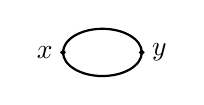
\begin{tikzpicture}[thick,scale=0.5] 
\filldraw (-1,0) circle (1pt) node[left] {$x$};
\filldraw (1,0) circle (1pt) node[right] {$y$};
\draw (0,0) circle (1cm and 0.6cm) ;
\end{tikzpicture}
\end{figure}
\end{minipage}
\hspace*{-8pt}
$\longrightarrow$
\hspace{5pt}
\begin{minipage}{0.7\linewidth}
\vspace*{-12pt}
\begin{equation*}
\Delta_\fsf^2(x,y) = \frac{1}{8 \pi^2} \bigg( \frac{u^2(x,y)}{\sigma_\fsf^2(x,y)} +  
\mbox{``well defined for $x=y$''}
\bigg)
\end{equation*}
\end{minipage}

\vspace*{10pt}

$\bullet$ regularize only $\sigma_\fsf^{-(2+\alpha)}$ \\

$\bullet$ use $\sigma$ identities : \ $ \Box \sigma = 4 + f \sigma $ \\
 
$\bullet$ $\alpha \mapsto \sigma_\fsf^{-(2+\alpha)}$ (weakly) meromorphic in $\alpha$. \\
\quad $\to$ Laurent series w.r.t $\alpha$ \\[-10pt]
\begin{equation*}
\frac{1}{\sigma_\fsf^{2+\alpha}}=\frac{1}{2\alpha(1+\alpha)}\left(\Box_x+(1+\alpha)f\right)\frac{1}{\sigma_\fsf^{1+\alpha}} 
\end{equation*}
\quad $\to$ subtract the principal part and take the limit $\alpha \to 0$ \\[-16pt]
%
\begin{equation*}
\left(\frac{1}{\sigma_\fsf^2}\right)_\mathsf{reg} \doteq \lim_{\alpha\to 0}\left(1-\pp\right)\frac{1}{M^{2\alpha}}\frac{1}{\sigma_\fsf^{2+\alpha}}=-\frac{1}{2}(\Box_x+f)\frac{\log M^2 \sigma_F}{\sigma_\fsf}-\Box_x \frac{1}{2\sigma_\fsf} 
\end{equation*}
%
\vspace*{-10pt}
%
\begin{equation*}
\Longrightarrow \ \left(\Delta_\fsf^{2}\right)_\mathsf{reg} 
\end{equation*}

\end{frame} 

%----------------------------------------------------------------------------%

\begin{frame}

\frametitle{PhD progress}
\framesubtitle{Summary}

\begin{exampleblock}{\vspace*{-3ex}}
\centering \textbf{BEFORE} \\ $\to$ conceptual well understanding of pAQFT on CST  
\end{exampleblock}
%
\vspace*{-8pt}
%
\begin{exampleblock}{\vspace*{-3ex}}
\centering \textbf{Problem} $\to$ $(\Delta_\fsf)^n, \dots $
\end{exampleblock}
%
\vspace*{-8pt}
%
\begin{exampleblock}{\vspace*{-3ex}}
\centering \textbf{regularisation procedure} $\to$ $(\Delta_\fsf)^{n} \ \simeq \ (\sigma_\fsf)^{-n} \ + \ \dots$ \\
with $(\sigma_\fsf^{-n})_{\mathsf{reg}} = \underset{\alpha \to 0}{\lim} \ (1-\pp) \ (\sigma_\fsf)^{-(n+\alpha)}, \ \alpha \in \Cbb$
\end{exampleblock}
%
\vspace*{-8pt}
%
\begin{exampleblock}{\vspace*{-3ex}}
\centering \textbf{NOW} \\ $\to$ computations accessible!
\end{exampleblock}
    
\end{frame} 

%----------------------------------------------------------------------------%
\section[Publi.]{Publication, preprint, in writing process}
%----------------------------------------------------------------------------%

\begin{frame}

\frametitle{Publication, preprint, in writing process}

A.~Géré, P.~Vitale, J.-C.~Wallet, \\
\titleref{Quantum gauge theories on noncommutative three-dimensional space}, \\
\PhysRevD{2014}{045019}{90}{10.1103/PhysRevD.90.045019},
\arxiv{hep-th}{1312.6145}{http://arxiv.org/abs/1312.6145}.\par
%
\bigskip
%
A.~Géré, J.-C.~Wallet, \\
\titleref{Spectral theorem in noncommutative field theories I: Jacobi dynamics}, \\
\arxiv{math-ph}{1402.6976}{http://arxiv.org/abs/1402.6976}.\par%
%
\bigskip
%
A.~Géré, T.-P.~Hack, N.~Pinamonti, \\
\titleref{Dimensional/Analytic regularisation on curved spacetime}, \\
in progress, to appear soon on \texttt{arxiv}.

\end{frame}  

%----------------------------------------------------------------------------%
\section[Conf.]{Scientific activities}
%----------------------------------------------------------------------------%

\begin{frame}
%
%
%
%
\frametitle{Scientific activities}
%
%
\begin{itemize}
% 
\item \textbf{Talks}
%
%
\begin{description}
\item - November 15th, 2014. \\ 
``Dimensional regularisation on curved spacetime'', \\
35th Local Quantum Pathroads Workshop, Goslar (Germany).
%
\item - December 11th, 2014. \\ 
Seminar of Mathematical Physics, LPT, Orsay (France).  
%
\end{description}
%
%
\item \textbf{Conferences Attended} \ 
%
%
\begin{description}
%
\item - November 14th -- 15th, 2014, \\ 
35th Local Quantum Pathroads Workshop, Goslar (Germany).
%
\item - October 29th -- November 2th, 2014, \\
Quantum Mathematical Physics, Regensburg (Germany).
%
\item - April 25th -- 26th, 2014, \\ 
34th Local Quantum Pathroads Workshop, Erlangen (Germany).
%
\end{description}
%
%
\end{itemize}
%
%
%
%
\end{frame}  

%============================================================================%
\end{document} 
%============================================================================%